\cleardoublepage\documentclass[../main.tex]{subfiles}
\begin{document}
\chapter{Aproximação Linear e o Método de Newton}\label{apend:MetNewton}

\section{Introdução}
Existem duas tarefas distintas para as quais você usa calculadoras científicas. Primeiro, elas realizam operações aritméticas básicas muito mais rapidamente do que qualquer um de nós poderia. Todos sabemos como multiplicar $1024$ por $1673$, por exemplo,  mas é demorado realizar esse cálculo com lápis e papel. Para esses problemas, as calculadoras são muito convenientes. Mais significativamente, também usamos calculadoras para calcular valores de funções transcendentais\footnote{Saiba mais  \href{https://pt.wikipedia.org/wiki/Função_transcendente}{neste link}} como seno, cosseno, tangente, exponencial e logaritmos. Nesse caso, a calculadora é muito mais que uma mera conveniência \cite{SmithCalculus}.


Como você calcularia $\sin(1.2345678)$ sem uma calculadora? Não se preocupe se você não sabe como fazer isso. O problema é que a função seno não é algébrica. Isto é, não existe uma fórmula para $\sin x$ envolvendo apenas as operações aritméticas. Então, como é que a sua calculadora “sabe” que $\sin(1.2345678) \approx 0 .9440056953$?  Em suma, não sabe disso  tudo. Em vez disso, \textit{a calculadora possui um programa embutido que gera valores aproximados de seno e outras funções transcendentais}.

Nesta seção, desenvolvemos um método simples de aproximação. Embora um pouco bruto, aponta o caminho para técnicas de aproximação mais sofisticadas.

\section{Aproximações Lineares}
Suponha que desejássemos encontrar uma aproximação para $f ( x_1 )$, onde $f (x_1)$ é desconhecido, mas onde
$f (x_0)$ é conhecido para algum $ x_0 $ ``próximo'' de $x_1$. Por exemplo, o valor de $\cos(1)$ é desconhecido, mas
sabemos que $\cos (\pi / 3) = 1/2$  e $\pi / 3 \approx 1,47$ é ``próximo'' de $1$. Embora pudéssemos usar $1/2$ como uma aproximação para $\cos (1)$, podemos fazer melhor.

Referindo-se à Figura \ref{fig:aproxLinearfx1}, observe que se $x_1$ está ``próximo'' de $x_0$ e seguimos linha  tangente
de $x = x_0$ para o ponto correspondente a $x = x_1$, então a coordenada $y $ desse ponto ($y_1$) deve estar ``próximo''  da coordenada $y$ do ponto na curva $y = f (x)$ [ou seja, $f (x_1)$].
\begin{figure}[H]
    \centering
    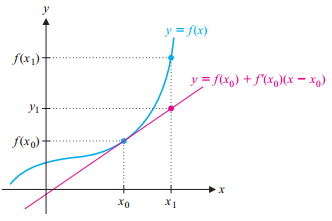
\includegraphics[scale=1.2]{fig_AproxLinear/AproxLinear-Fx1.png}
    \caption{Aproximação linear de $f(x_1)$}
    \label{fig:aproxLinearfx1}
\end{figure}
Como a inclinação da reta tangente a $y = f (x)$ em $x = x_0$ é \(f'(x_0)\), a equação da reta tangente a $y = f (x)$ em $x = x_0$ é encontrada de
\begin{equation}
m_{tan}=f'(x_0)=\frac{y-f(x_0)}{x-x_0}\label{eq:CoefAngRetTang}
\end{equation}
Resolvendo a equação (\ref{eq:CoefAngRetTang}) para $y$, encontramos:
\begin{equation}
    y=f(x_0)+f'(x_0)(x-x_0)\label{eq:AproxLinear}
\end{equation}

Observe que (\ref{eq:AproxLinear}) é a equação da reta tangente ao gráfico de $y = f (x)$ em $x = x_0$. Vamos nomeá-la na definição a seguir.
\begin{definition}\label{def:AproxLinear}
A aproximação linear (ou linha tangente) de $f (x)$ em $x = x_0$ é a função $$L(x)=f(x_0)+f'(x_0)(x-x_0)$$
\end{definition}

Observe que a coordenada y ($y_1$) do ponto na reta tangente correspondente a $x = x_1$ é simplesmente encontrado substituindo $x = x_1$ na equação (\ref{eq:AproxLinear}). Isso nos dá
\begin{equation}
    y_1=f(x_0)+f'(x_0)(x_1-x_0)\label{eq:AproxLinear-y1}
\end{equation}

Considerando   $\Delta x=x-x_0\Rightarrow x=x_0+\Delta x$ na equação (\ref{eq:AproxLinear}), podermos reescrevê-la como segue:
\begin{equation}
    f(x_0+\Delta x)\approx f(x_0)+f'(x_0)\Delta x\label{eq:aproxDerivada}
\end{equation}
Observe que a equação (\ref{eq:aproxDerivada}) é equivalente a $f'(x_0)\approx \frac{f(x_0+\Delta x)-f(x_0)}{\Delta x}$ que é  a aproximação da derivada da função $f$ no ponto $x=x_0$.
\begin{ex}
Encontre a aproximação linear de $f (x) = \cos x$ em $x_0 = \pi / 3$ e use-a para aproximar $\cos (1)$.
\end{ex}
\begin{sol}
Na definição \ref{def:AproxLinear}, a aproximação linear é definida como
$$L(x)=f(x_0)+f'(x_0)(x-x_0)$$
Temos que $x_0 = \pi / 3, f (x) = \cos x$ e $f'(x) = - \sin x$. Então nós temos 
$$L(x)=\cos\pc{\frac{\pi}{3}}-\sin\pc{\frac{\pi}{3}}\pc{x-\frac{\pi}{3}}=\frac{1}{2}-\frac{\sqrt{3}}{2}\pc{x-\frac{\pi}{3}}$$

Observe que escolhemos $x_0 = \pi/3$ desde $\pi/3$ é o valor mais próximo de $1$ no qual sabemos o valor exato do cosseno. Finalmente, uma estimativa para $\cos (1)$ é 
$$L(1)=\frac{1}{2}-\frac{\sqrt{3}}{2}\pc{1-\frac{\pi}{3}}\approx 0,5409$$

Sua calculadora fornece $\cos (1) \approx 0,5403$ e, portanto, descobrimos uma aproximação ao valor desejado.
 
\end{sol}
No exemplo \ref{ex:AproxSINX}, derivamos uma aproximação útil para $\sin x$, válida para $x$ próximo a $0$. Essa  aproximação é frequentemente usada em aplicações em física e engenharia para simplificar equações envolvendo $\sin x$.

\begin{ex}\label{ex:AproxSINX}
Encontre a aproximação linear de $f (x) = \sin x$, para $x$ próximo a $0$.\\
\begin{sol}
$f(x) =\cos x$, de modo que, na definição \ref{def:AproxLinear}, temos
$$\sin x \approx L (x) = f (0) + f'(0) (x - 0) = \sin 0 + \cos 0\cdot  (x) = x$$
Isso significa que para $x$ próximo a $0$, $\sin x \approx x$. Ilustramos isso na Figura \ref{fig:y=sinx-y}, onde mostramos
gráficos de ambos $y = \sin x$ e $y = x$.
\begin{figure}[H]
    \centering
    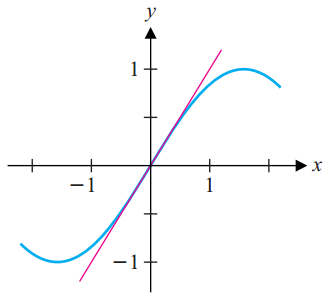
\includegraphics{fig_AproxLinear/sinxy=x.png}
    \caption{$y=\sin x$ e $y=x$}
    \label{fig:y=sinx-y}
\end{figure}

Observe na Figura \ref{fig:y=sinx-y} que o gráfico de $y = x$ permanece próximo ao gráfico de $y = \sin x$ somente nas proximidades de $x = 0$. Assim, a aproximação $\sin x \approx x $ é válida apenas para $x$ próximo a $0$.    
\end{sol}
\end{ex}
\begin{ex}\label{ex:AproxRaiz}
Vamos utilizar a fórmula \ref{eq:AproxLinear} para determinar $\sqrt{12}$, utilizando como aproximação inicial o número $3$, já que o quadrado perfeito mais próximo do número $12$ é o número $9$ e $3=\sqrt{9}$.
\begin{sol}
Sendo $f(x)=\sqrt{x}$ então $f'(x)=\frac{1}{2\sqrt{x}}$. Considerando $x_0=3$ e $\Delta x=12-9=3$ na equação (\ref{eq:aproxDerivada}), temos:
\begin{align*}
    f(x+\Delta x)\approx f(x_0)+f'(x_0)\Delta x\\
    \sqrt{9+3}\approx\sqrt{9}+\frac{3}{2\sqrt{9}}\\
    \sqrt{12}\approx3+\frac{3}{6}=3,5
    \end{align*}
Assim, encontramos a aproximação $3,5$ para a $\sqrt{12}$. Se elevarmos o número $3,5$ ao quadrado, encontramos o valor de $12,25$. Portanto, temos um erro de $12,25-12=0,25$. Na próxima seção abordaremos o método de Newton que nos fornece uma aproximação melhor para tais cálculos.
\end{sol}
\end{ex}
\begin{obs}
 Apesar do método da aproximação linear não ser tão preciso, conforme vimos no exemplo anterior, ele é extremamente útil para entendermos métodos mais eficazes. Quanto menor o valor de $|\Delta x|$ mais preciso será o cálculo do método de aproximação linear. Isto nos instrui a procurar o número que tem raiz exata mais próxima para tomar como $x$. Se tomássemos por exemplo $x=16$ e $\Delta x=-4$ (já que $12=16-4)$, o resultado seria menos preciso já que o número $16$ está mais distante do número $12$ do que o número $9$. Mas se quiséssemos, por exemplo, $\sqrt{15}$, seria melhor utilizar $x=16$.
\end{obs}
\begin{obs}
 Para uma melhor aproximação do cálculo do exemplo \ref{ex:AproxRaiz}, podemos aplicar o método da aproximação linear novamente utilizando $x_0=3,5$ e $\Delta x=(3,5)^2-12=12,25-12=0,25$, conforme resultado  obtido, como segue:
 \begin{align*}
    f(x+\Delta x)\approx f(x_0)+f'(x_0)\Delta x\\
    \sqrt{12}=\sqrt{12,25-0,25}\approx \sqrt{12,25}- \frac{0,25}{2\sqrt{12,25}}\\
    \sqrt{12}\approx 3,5-\frac{3,5}{7}=3,5-0,036=\pmb{3,464}
    \end{align*}
    Esta última aproximação é muito melhor que a primeira e é a mesma aproximação com três casas decimais fornecidas pelas calculadoras.
\end{obs}
\section{Método de Newton}
  Para resolver equações de grau menor que 3 temos métodos analíticos, fácies de serem aplicados, tais como a ``Fórmula de Bháskara'':  $x=\frac{-b\pm\sqrt{b^2-4ac}}{2a}$. No caso de equações de grau três, apesar de existirem métodos analíticos para resolvê-las, os mesmos são complicados de se trabalhar, o que compensa mais trabalhar com métodos numéricos de aproximação das soluções. Para equações de grau maior que 3, temos que recorrer indispensavelmente a métodos numéricos. A seguir apresentaremos um destes métodos desenvolvido pelo físico Isaac Newton\footnote{Saiba mais sobre \href{https://pt.wikipedia.org/wiki/Isaac_Newton}{Isaac Newton}}.

Considere a equação cúbica 
\begin{equation}
    x^3 - 3x- 5 = 0\label{eq:cubica}
\end{equation}
 denotando $x^3 - 3x- 5 = 0$ por $f(x)$, poderemos calcular facilmente os seguintes valores: 
$$f(- 2) =-7, f(- 1)=-3, f(0) =- 5, f(1) =-7, f(2) =-3, f(3) =1 3$$ 
O par de valores $f(2) = - 3$ e $f(3) = 13$ sugere que, quando $x$ varia continuamente de $2$ a $3$, $f(x)$ varia continuamente de $-3$ a $13$ e que, consequentemente, existe algum valor de $x$ entre 2 e 3 tal que $f(x) = 0$. Lembremos que:  se uma função contínua $f(x)$ tem valores $f(a)$ e $f(b)$ com sinais opostos, então existe pelo menos uma raiz da equação $f(x) = 0$ entre $a$ e $b$. Assim a equação (\ref{eq:cubica}) tem uma raiz entre $x = 2$ e $x = 3$ e podemos tomar um desses números como uma \textbf{primeira} aproximação da raiz. A aproximação $x = 2$ é a melhor escolha, pois -3 esta mais próximo de 0 que 13. 

Suponhamos agora, generalizando, que temos uma primeira aproximação $$x = x_0$$ de uma raiz $r_1$ da equação $f(x ) =0$. Essa raiz é um ponto em que a curva $y = f(x )$ ``atravessa'' (intercepta) o eixo $x$ (Fig. \ref{fig:MetNewon}). 
\begin{figure}[H]
    \centering
    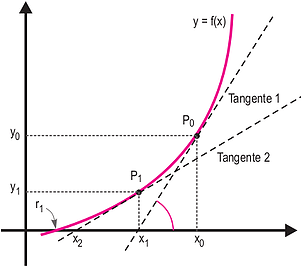
\includegraphics[scale=0.6]{fig_MetNewton/MetNewton.png}
    \caption{Ilustração do Método de Newton}
    \label{fig:MetNewon}
\end{figure}

A ideia do método de Newton é usar a reta tangente a curva no ponto \( x = x_0 \) tomando-o como 
ponto de partida para uma melhor aproximação \(x = x_1\).  Começando com a aproximação \( x = x_0 \), 
desenhamos a reta tangente a curva no ponto $(x_0,f(x_0))$. Essa reta intercepta o eixo \(x\) no ponto 
\(x = x_1\), que, em geral, é uma melhor aproximação do que $x_0$.  Repetindo esse processo, usamos 
a reta tangente em \((x_1, f(x_1 ))\) para obter o ponto \(x =x_2\), que é uma aproximação ainda melhor. 
A Fig. \ref{fig:MetNewon} ilustra a ideia como procedimento geométrico, mas para aplicá-la nos cálculos precisamos de uma fórmula. Essa fórmula é obtida facilmente como se segue. 

O coeficiente angular da primeira tangente é $f'(x_0)$. Se considerarmos essa reta como sendo determinada pelos pontos $(x_1, 0)$ e $(x_0,f(x_0))$, conforme figura \ref{fig:MetNewon}, então o coeficiente angular será também: 
\matt{ f'(x_0) =\frac{0-f(x_0)}{x_1-x_0}}
Essa equação leva a
\begin{equation*}
     x_1-x_0=-\frac{f(x_0)}{f'(x_0)}
\end{equation*}
ou equivalentemente
\begin{equation}
   x_1=x_0-\frac{f(x_0)}{f'(x_0)}
    \label{eq:segAprox}
\end{equation}

Dessa maneira, partindo de nossa 1ª aproximação $x_0$ obteremos a 2º aproximação $x_1$ por meio 
de (\ref{eq:segAprox}); esta, por sua vez, leva a uma 3ª aproximação $x_2$, dada por 
\begin{equation}
   x_2=x_1-\frac{f(x_1)}{f'(x_1)}
    \label{eq:tercAprox}
\end{equation}
e assim por diante, indefinidamente. Assim, podemos generalizar o \textbf{Método de Newton}, conforme segue:
\begin{equation}
 \boldsymbol{ x_{n+1}=x_{n}-\frac{f(x_n)}{f'(x_n)}} \textrm{ para } n=0,1,2,3, \ldots \label{eq:MetNewton}
\end{equation}

Ao aplicar esse método a equação (\ref{eq:cubica}), temos 
\matt{f(x)=x^3 - 3x- 5, \qquad f'(x)=3x^2-3\qquad x_0=2,
}
\matt{f(x_0)=-3, \qquad f'(x_0)=9\qquad x_1=x_0-\frac{f(x_0)}{f'(x_0)}=2-\frac{-3}{9}=\frac{7}{3}\approx \pmb{2,33}
}

Vamos agora ao cálculo de $x_2$ (terceira aproximação):
\matt{f(x_1)=f\pc{\frac{7}{3}}=\frac{19}{27}, \qquad f'(x_1)=f'\pc{\frac{7}{3}}=\frac{40}{3}
}
\matt{x_2=x_1-\frac{f(x_1)}{f'(x_1)}=\frac{7}{3}-\frac{\frac{19}{27}}{\frac{40}{3}}=\frac{7}{3}-\frac{19}{27}\cdot \frac{3}{40}=\frac{7}{3}-\frac{19}{360}=\frac{821}{360}\approx \pmb{2,28}
}

Para impedir que nossos cálculos fiquem por demais penosos, nos satisfaremos com duas casas decimais de precisão. Quando duas aproximações sucessivas forem iguais em suas duas  primeiras casas decimais, consideraremos o fato como uma evidencia de termos chegado ao resultado com tal precisão. Por exemplo, no caso da equação (\ref{eq:cubica}), obtivemos $2,28$ como uma 
aproximação da raiz após duas aplicações da equação (\ref{eq:MetNewton}). Uma outra aplicação  da equação (\ref{eq:MetNewton}) leva ao 
mesmo número $2,28$. Concluímos portanto que $2,2$8 é uma raiz da equação (\ref{eq:cubica}), que é precisa em duas casas decimais. Obviamente que se quisermos aproximações com número maior de casas decimais, obteremos soluções mais precisas. Tudo depende de quanto laborioso serão os cálculos e de qual meio para executá-los você utilizará.


O \textbf{Método de Newton} não se restringe a solução de equações polinomiais como (\ref{eq:cubica}), mas também pode ser aplicado a qualquer equação contendo funções cujas derivadas podemos calcular. Entretanto, por simplicidade, nos problemas dados aqui concentramos nossa atenção nos polinômios. 

\begin{obs}
 Em alguns casos, a sequência das aproximações produzida pelo método de Newton pode deixar de convergir para a raiz procurada, em particular se a derivada da função no ponto for nula. A teoria matemática explicitando as condições 
nas quais se garante que o método de Newton seja bem-sucedido pode ser encontrada em livros de cálculo numérico. 
\end{obs}

\begin{exeresol}
Vamos utilizar o método de Newton para calcular $\sqrt{12}$ , afim de comparação com o Exemplo \ref{ex:AproxRaiz}.
\end{exeresol}
\begin{sol}
Lembre-se de que podemos usar uma aproximação linear para fazer isso. Por outro lado,
O método de Newton é usado para resolver equações da forma $f (x) = 0$. Podemos reescrever o
problema suponho que $x = \sqrt{12}$. Então, $x^2 = 12$, que pode ser reescrito como $$f(x)=x^2-12=0$$
Utilizaremos  $x_0=3$ como primeira aproximação, temos:
\begin{align*}
   f(x_0)=-3 &\qquad\qquad f(x)=2x &f'(x_0)=6
\end{align*}
Segue que
\begin{align*}
     x_1=x_0-\frac{f(x_0)}{f'(x_0)}\\
     x_1=3-\frac{-3}{6}=3+\frac{1}{2}=3,5
\end{align*}
O resultado da primeira interação nos deu o mesmo resultado obtido no Exemplo \ref{ex:AproxRaiz}. Vamos a segunda iteração, considerando $f(3,5)=(3,5)^212=0,25$ e $f'(3,5+=2\cdot 3,5=7$
\begin{align*}
     x_2=x_0-\frac{f(x_1)}{f'(x_1)}\\
     x_2=3,5-\frac{0,25}{7}=3,5-0,036=\pmb{3,464}
\end{align*}
Este resultado também bate com o resultado obtido na segunda aplicação do método de aproximação linear para o exemplo em questão. No entanto, nem sempre isso irá acontecer, na maioria dos casos, o método de aproximação linear por não ser um método iterativo, sempre fornece uma aproximação menos precisa do que o método de Newton, mesmo aplicado repetidas vezes. Veja o exercício resolvido \ref{exer:RaizCubica}
\end{sol}
\begin{exeresol}\label{exer:RaizCubica}
Utilize o método de Newton para aproximar $\sqrt[3]{7}$
\end{exeresol}
\begin{sol}
 Podemos reescrever o problema suponho que $x = \sqrt[3]{7}$. Então, $x^3 = 7$, que pode ser reescrito como $$f(x)=x^3-7$$.\\
 Temos que $f'(x) = 3 x^ 2$ e podemos tomar como aproximação inicial $x_0=2$. Neste caso, segue que\\
 $$x_1=2-\frac{1}{12}=\frac{23}{12}\approx 1,916666667$$\\
 Continuando o processo, temos:
 $$x_2\approx 1,912938458$$
 $$x_3\approx 1,912931183\approx x_4$$
 Por outro lado,
 $$f(x_4)\approx 1\times 10^{-13}$$
 e assim, $x_4$ é um zero aproximado de $f$. Isso também diz que
 $$\pmb{\sqrt[3]{7}\approx 1,912931183}$$
 que se compara muito favoravelmente com o valor de $\sqrt[3]{7}$ fornecido pela sua calculadora.
 
 Se tivéssemos usado o método de aproximação linear encontraríamos como resposta $1,75$ que é uma aproximação muito menos precisa do que a que foi encontrada no Método de Newton na primeira iteração.
\end{sol}
\begin{obs}
Para obtermos resultados cada vez mais precisos é preciso irmos comparando o resultado de $f(x_{n+1})$ obtido pela equação \ref{eq:MetNewton} com o número $0$, quanto mais próximo estiver $|f(x_{n+1})|$ de zero mais preciso é a solução encontrada, uma vez que para a raiz exata, tem-se $f(x)=0$.
\end{obs}
\subsection*{Exercícios}
\begin{exer}
Esboçando o gráfico de \(y = f(x) = x^3 - 3x - 5\), mostre que a equação (\ref{eq:cubica}) tem somente uma raiz real. \textbf{Sugestão:} use a derivada\( f'(x) = 3x^2 - 3 = 3(x^2 - 1)\) para localizar os máximos e mínimos da função e saber onde é crescente e decrescente. 
\end{exer}
\begin{exer}~
\\ (a) Mostre que $x^3 + 3x^2 - 6 = 0$ tem somente uma raiz real e calcule-a com duas casas decimais de precisão. \\
(b ) Mostre que $x^3 + 3x = 8$ tem somente uma raiz real e calcule-a com duas casas decimais de precisão. 
\end{exer}
\begin{exer}\label{probanterior}
 Use o método de Newton para calcular a raiz positiva de $x 2 + x-1 = 0$ com duas casas decimais de precisão.
\end{exer}
\begin{exer}
Calcule $\sqrt{5}$ com duas casas decimais de precisão, resolvendo a equação $x^2 - 5 = 0$ e use esse resultado  na formula quadrática para conferir a resposta do Problema \ref{probanterior}. 
\end{exer}
\begin{exer}
Use 0 método de Newton para calcular $\sqrt[3]{10}$ com duas casas decimais de precisão. 
\end{exer}























\end{document}